\documentclass{article}
\usepackage{graphicx}
\usepackage[british]{babel}
\usepackage{ams math}
\usepackage[utf8]{inputenc}
\usepackage[official]{eurosym}
\DeclareUnicodeCharacter{20AC}{\euro{}}
\usepackage{color}
\usepackage{listings}
\usepackage[hidelinks]{hyperref}
\usepackage[a4paper]{geometry}
\usepackage{fullpage}
\usepackage{fancyhdr}


\title{PowerGAMA\\User guide (v1.0.2)}
\author{Harald G Svendsen}
\date{\today}

\fancyhf{}
\renewcommand{\headrulewidth}{0pt}
\rhead{
	\setlength{\unitlength}{1mm}
	\begin{picture}(0,0)
      	\put(-15,-15){
\includegraphics[width=40mm]{logo_condensed.png}}
	\end{picture}
}
\pagestyle{fancyplain}


\begin{document}

\maketitle

\begin{abstract}
This document gives a rough and brief overview of the PowerGAMA software tool for optimal power flow analysis of large power systems, taking into account variability of demand and power generation from renewable sources.
\end{abstract}

\tableofcontents


\newpage
\section{Introduction}
PowerGAMA is open source software created by SINTEF Energy Research. The expanded name is \emph{Power Grid And Market Analysis}. This is a Python-based  lightweight simulation tool for high level analyses of renewable energy integration in large power systems.

The simulation tool optimises the generation dispatch, i.e. the power output from all generators in the power system, based on marginal costs for each timestep for a given duration.  It takes into account the variable power available for solar, hydro and wind power generators. It also takes into account the variability of demand. Moreover, it is flow-based meaning that the power flow in the AC grid is determined by physical power flow eqautions. 

Since some generators may have an energy storage (hydro power with reservoir and consentrated solar power with thermal storage) the optimal solution in one timestep depends on the previous timestep, and the problem is  therefore be solved sequentially.  A realistic utilisation of energy storage is ensured through the use of storage values.


PowerGAMA does not include any power market subtleties (such as start-up costs, limited ramp rates, forecast errors, unit commitments) and as such will tend to overestimate the ability to accomodate large amounts of variable renewable energy. Essentially it assumes a perfect market based on nodal pricing without barriers between different countries. This is naturally a gross oversimplification of the real power system, but gives nontheless very useful information to guide the planning of grid developments and to assess broadly the impacts of new generation and new interconnections.

PowerGAMA is largely inspired by SINTEF's Power System Simulation Tool (PSST) 
\cite{korpas2007,hueartas2010}.

\bigskip\noindent
PowerGAMA source code and a wiki is found on this web address:
\\ 
\url{https://bitbucket.org/harald_g_svendsen/powergama}.

\subsection{Licence}
PowerGAMA is open source software distributed under the following licence:
\begin{itemize}
\item The MIT License (MIT) (\url{http://opensource.org/licenses/MIT})
%\item Mozilla Public License 2.0 (MPL-2.0)
%\item GNU General Public License, version 3 (GPL-3.0)
\end{itemize}

\subsection{Dependencies}
PowerGAMA is written with Python, and is executed via a Python interpreter.
It has the following dependencies, all of which are freely available:

\begin{itemize}
\item Python 3 or 2.7
\item Python packages: numpy, scipy, matplotlib, mpl\_toolkits, PuLP
\end{itemize}

\subsection{Installation}

The above dependencies must be installed before PowerGAMA can be executed. Convenient Python packages that includes the numpy, scipy and matplotlib packages and the Matlab-like development environment Spyder are \emph{Anaconda} () and \emph{Python(x,y)}.
%
Installing additional python packages is generally straightforward, using e.g. \emph{pip} or the "python setup.py install" command. This includes the installation of PowerGAMA itself.




\section{Physical description}

This section gives a brief overview of the physical description of the power system grid and market. This description includes a number of implicit assumptions and is the basis for the PowerGAMA software tool.



\subsection{Electricity market}
The market is considered perfect such that generators with the lowest marginal costs are always favoured. That is, power is assumed traded such that the overall cost of generation is always minimised.

The cost of generation is assumed to be the marginal cost times power output for all generators. Start-up costs and ramp rates are not considered.

For generators with a storage, the marginal cost is given by storage values, which depends on filling level.
Storage values are inspired by watervalues used for modelling and planning of production for hydro power generators with storage \cite{fosso1999,wolfgang2009}. Storage values reflect the value of adding power inflow to the storage. The generator will therefore produce if the cost of alternative generation is higher than the storage value at any given time. This is identical to saying that a generator with storage will produce powr if the nodal price is higher than the storage value.

Storage values curves are given as input, as functions of storage filling level and time.
If the storage is nearly full, the storage value is low, since adding to the storage may lead to energy spillage. If the storage is nearly empty, the storage value is high. 
For predictable seasonal or daily inflow patterns, the storage value is low just before a peak in the inflow,  and high before a dip. An illustration of how the storage values may vary with filling level and time is given in Figure~\ref{fig:storagevalues} for solar consentrated power with small storage (hours) and for hydro power with large reservoir for seasonal storage.


\begin{figure}
\centering
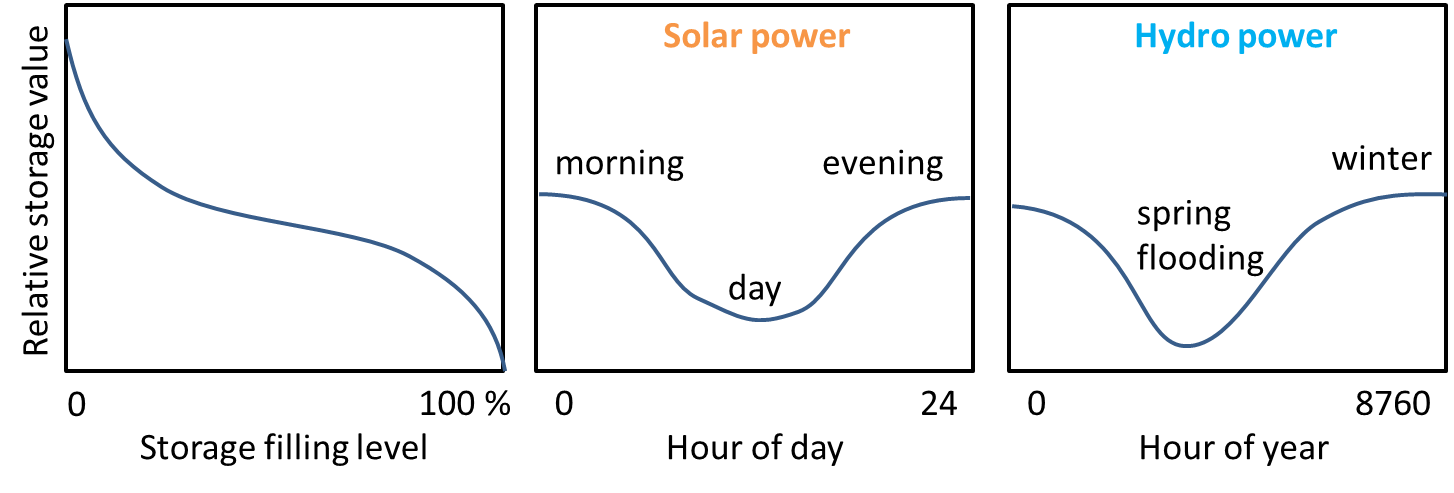
\includegraphics[scale=0.6]{storagevalues.png}
\caption{Illustration of typical storage values with dependence on filling level (left) and time variation for solar power with small storage (middle) and hydro with large storage (right)}
\label{fig:storagevalues}
\end{figure}



\subsection{Power generation}

\begin{figure}
\centering
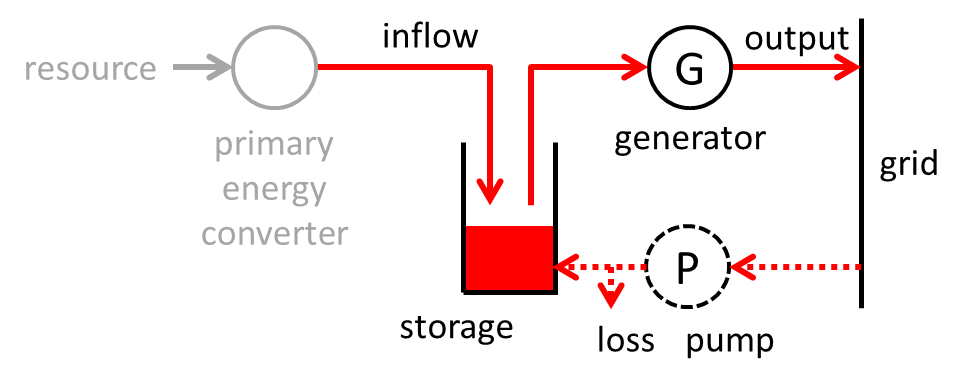
\includegraphics[scale=0.6]{generator_model4.png}
\caption{Power generation model model.}
\label{fig:generator_model}
\end{figure}

\begin{table}
\caption{Generator parameters: Inflow, storage capacity and marginal cost for different types of generators}
\label{tab:generator_parameters}
\begin{tabular}{llll}
\hline
Generator type & Inflow & Storage & Price \\ 
\hline
Fuel based (alt 1) & 0 & Infinity & Constant cost \\
Fuel based (alt 2) & Available capacity & 0 & Constant cost\\
Wind & Available power & 0 & 0 \\
Photovoltaic & Available power & 0 & 0 \\
CSP & Available power & Thermal storage & Storage value \\
Hydro & Water inflow & Reservoir capacity & Storage value \\
\hline
\end{tabular}
\end{table}

Power generators are described by the same universal model, illustrated in Figure~\ref{fig:generator_model}.
Different types of power plants are simply distinguished by their different parameters, as indicated in Table~\ref{tab:generator_parameters}.
PowerGAMA assumes that the power inflow (average value and time profile) is given as input, and so the resource and primary energy converter parts included in Figure~\ref{fig:generator_model} are not directly relevant. 

Wind and solar PV power are similar. The inflow represents the available electrical power in the wind or solar radiation. Zero storage implies that power not used is lost.  The cost is zero, such that unless restricted by grid constraints, available power will always be output.
solar CSP and hydro power \emph{without} any storage can also be modelled in this way.

CSP and hydro \emph{with storage} will have a non-zero storage and a price set such as to ensure a sensible scheduling of the power output. If the storage is close to its upper limit, the price will be low and if it is low, the price will be high. This dependence on the storage filling level is exactly what the storage value provides. It gives the threshold price value for when the generator should produce power at a given storage filling level. The use of storage value is well established for scheduling of hydro power production.
Storage values also depend on the time: The value of stored water is less just before the spring floods than in the autumn, and the value of stored CSP energy is less in the late morning (around 9am) than in the evening. However, this dependence will be ignored in this software.

For fuel based generators, such as coal, gas, oil, nuclear and biomass, there are two alternative ways to specify the inflow and storage parameters. 
\emph{Alternative One} is to set inflow to zero and storage to infinity with an initial value also to infinity. Then there is always fuel available in the storage and output is restricted by generator output limits only.  With this approach there is no spilled energy, but storage is updated each time step.
\emph{Alternative Two} is to set inflow equal to available capacity and storage to zero. This allows available capacity to vary throughout the year, which may be relevant at least for nuclear power and perhaps biomass. But it will wrongly indicate spilled energy whenever actual output is less than the available capacity.


%This model may easily be extended to include pumping/charging capacity (with an energy loss), but this will not be done now.
For generators with a storage, a pump, or more generally, an energy storage charger, may be included in the model. Technically, a pump is represented as a generator with zero or negative output that takes energy from the grid and adds to the storage, with a certain amount of loss.

The generator model is described by the following parameters:
\begin{itemize}
\item Power inflow ($P_\text{inflow}$)
\item Energy storage capacity ($E_\text{max}$)
\item Energy in storage ($E$)
\item Generator capacity ($P_\text{max}$)
\item Generator minimum production ($P_\text{min}$). Normally, this is value is zero.
\item Generator output ($P_\text{output}$)
\item Generator available power ($P_\text{avail}$)
\item Pumping capacity ($P_\text{pump,max}$). In most cases, this value is zero (no pumping)
\item Pumping demand ($P_\text{pump}$)
\item Pumping efficiency ($\eta_\text{pump}$)
\end{itemize}

Available power is determined by the power inflow and the amount of stored energy, and is given by
\begin{equation}
	 P_\text{avail} = P_\text{inflow} + \frac{E}{\Delta t},
\end{equation}
where $\Delta t$ is the time interval considered.

Generator output is limited both by the available power and by the generator capacity, as well as the minimum production. Regarding the upper limit, there is a difference depending on generator type.
%
From the definition of power capacity for PV panels, it may occur in good conditions that the power output is higher than the nominal capacity. In this case output power should not be constrained by the nominal capacity, but only by the available power.  In fact, this is true for all generators with zero storage. 
In general, therefore, the upper limit on generator output is given as
\begin{eqnarray}
	\text{No storage generators:} \quad && P_\text{limit} = P_\text{avail},
	\\
	\text{Non-zero storage generators:} \quad && P_\text{limit} = \min[P_\text{avail}, P_\text{max}],
	\\
	\text{Infinite storage generators:} \quad && P_\text{limit} = P_\text{max}.
\end{eqnarray}
The constraint on generator power output can then be written
\begin{equation}
	 P_\text{min} \le P_\text{output} \le P_\text{limit}.
\end{equation}




\subsubsection{Power inflow}
Power inflow is important for renewable energy sources such as wind, sun and rain. In general the energy resource may be converted by a primary energy converter (e.g. wind turbine) into a more readily exploitable energy form. The available power for electricity generation is generally less than the power in the primary resource.  PowerGAMA assumes that power inflow data is provided by the user.
For wind power, the inflow depends on the wind speed and characteristics of the wind turbines.
Similarly, for solar power the inflow depends on solar radiation and characteristics of the PV or CSP units.
For hydro power, the inflow depends on precipitation, temperature, topography and soil conditions.


\subsubsection{Pumping}
\begin{figure}
\centering
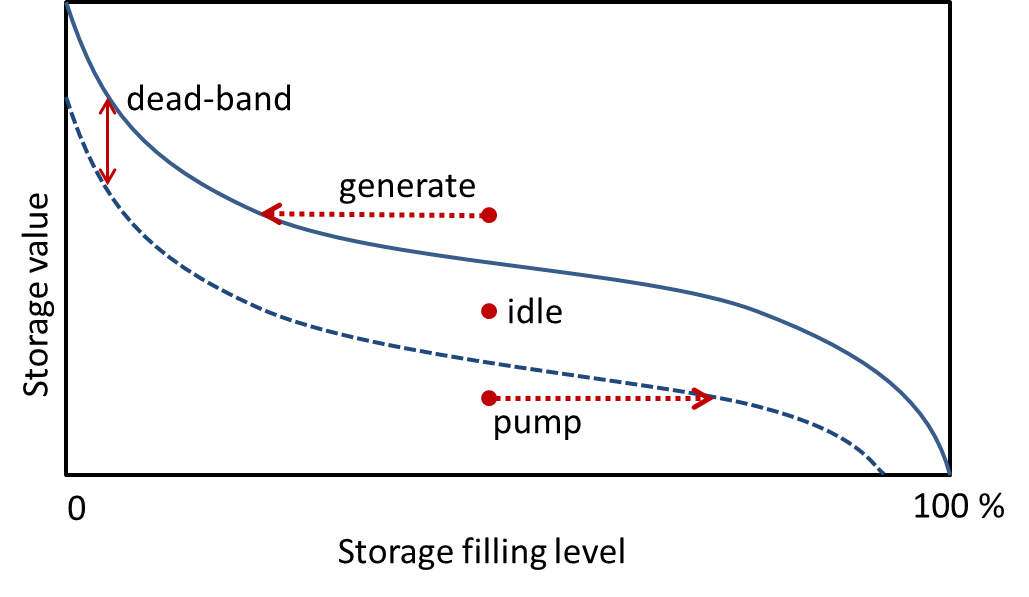
\includegraphics[scale=0.6]{generate_idle_pump2.png}
\caption{Generator with storage and pumping. The red dots represent three different situations with different nodal price at the generator associated node. The solid line is the storage value curve, and the dotted line is the same curve offset by a dead-band.}
\label{fig:pumping_model}
\end{figure}

The implementation of pumping is illustrated in Figure~\ref{fig:pumping_model}.
If the price is high, the generator will produce power, reducing the storage filling level. If the price is below the storage value the generator will be idle, allowing the storage to fill up (due to inflow). If the price is also lower than the storage value minus a certain dead-band value, the pump will add energy to the storage, increasing the filling level.

The dead-band ensures that the generator--pumping system doesn't continuously alternate between generating and pumping, and indirectly takes into account the losses associated with pumping.


\subsubsection{Storage dynamics}

The energy in the storage $E$ is given by the differential equation
\begin{equation}
	\frac{dE}{dt} = P_\text{inflow} - P_\text{output} + \eta_\text{pump}P_\text{pump}, 
	\quad 0 \le E \le E_\text{max},
\end{equation}
where $E_\text{max}$ is the maximum capacity of the storage. Discretised, this equation is written
\begin{equation}
	E(t+\Delta t) = \max[\min[E(t) 
	+ \Delta t (P_\text{inflow} - P_\text{output} + P_\text{pump}), 
	E_\text{max})],0]
\end{equation}




\subsection{Power consumption}

Power consumption is modelled as loads connected to different nodes with a given average power demand and a certain profile which describes the time dependent variation, i.e. how the power consumptions varies from time step to time step. Any number of demand profiles can be specified and any number of loads can be connected to each node.

The full consumption model is illustrated in Figure~\ref{fig:load_model}, with futher explanaitions in the following.


\begin{figure}
\centering
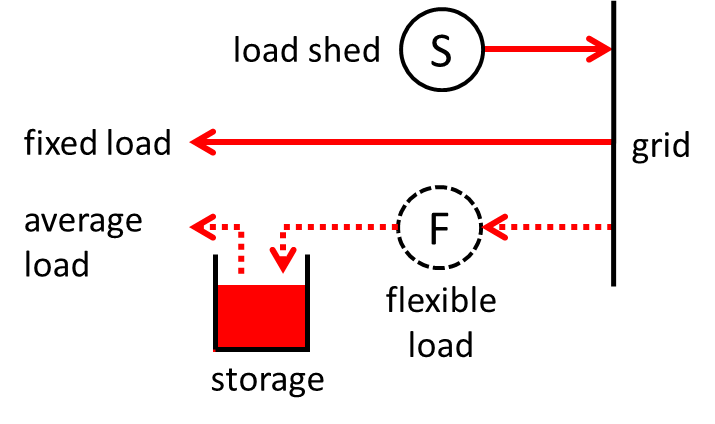
\includegraphics[scale=0.6]{load_model.png}
\caption{Power consumption model.}
\label{fig:load_model}
\end{figure}

\subsubsection{Load shedding}
Power demand that for some reason cannot be supplied is handled by adding high cost generators at all nodes with loads attached. This ensures that the optimisation has a solution.
The high cost further ensures that these are used only when strictly necessary. Output from these ``generators'' is interpreted as load shedding.

\subsubsection{Flexible load}
Flexible loads are represented in a similar way to flexible generation, by means of a storage and storage value curves. 

The main parameters specifying a flexible load are:
\begin{itemize}
\item The ratio of flexible energy to total energy demand ($P_\text{flex}^\text{avg}/P^\text{avg}$)
\item The flexibility on/off ratio, i.e. ratio of average load  relative to the maximum load ($x_\text{flex} = P_\text{flex}^\text{avg} / P_\text{flex}^\text{max}$)
\item The maximum energy flexibility/storage ($E_\text{flex}^\text{max}$), given in MWh
\item The storage value curve (normalised shape)
\item The storage base value (absolute value), given in €/MWh
\end{itemize}
%
%From the total average load $P^\text{avg}$, the average flexible load is calculated as 
%
%The maximum power that can be supplied to the flexible load is
%$P_\text{flex}^\text{max} = P_\text{flex}^\text{avg}/x_\text{flex}$.

The amount of power served to the flexible load, $P_\text{flex}$ is determined by the optimisation. Given this value, the energy in the storage $E_\text{flex}$ for the flexible load is computed according to
\begin{equation}
	 E_\text{flex}(t+\Delta t) = E_\text{flex}(t) + \Delta t (
		P_\text{flex}-P_\text{flex}^\text{avg} ),
\end{equation}
where $\Delta t$ is one time step.
The storage filling level $f_\text{flex}$ is the relative value of energy in the storage compared to the maximum flexible energy (storage capacity),
\begin{equation}
	f_\text{flex} =  \frac{E_\text{flex}}{E_\text{flex}^\text{max}}.
\end{equation}
If $f_\text{flex}>0.5$ then the load is ``over-served'', and 
if $f_\text{flex}<0.5$ then it is ``under-served''.
It is assumed that the initial value of the filling level is 0.5.

Flexibility value curves specify flexibility values as functions of flexibility status. This is akin to storage values versus filling level for storage generators.
An example of such a curve is shown in Figure~\ref{fig:flexvalue_curve}.
If the associated nodal price is lower than the flexibility value, then the load is served. This in turn increases the flexibility status.


\begin{figure}
\centering
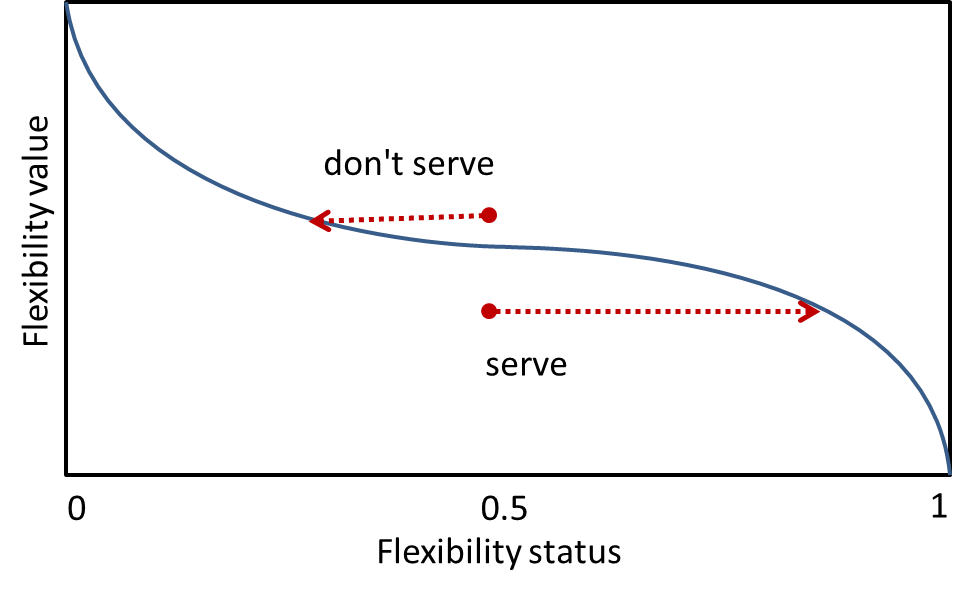
\includegraphics[scale=0.6]{flexvalues.png}
\caption{Storage value curve for flexible load. The red dots represent nodal prices in two different operating points }
\label{fig:flexvalue_curve}
\end{figure}




\subsection{Grid power flow}

The power balance at each node  requires that all generation minus all consumption equals the net power flow \emph{out} of the node. Additionally, AC power flow in the grid obeys power flow equations, and is moreover constrained by capacity limits. These physical relationships and constraints can be formulated  by a set of equations and inequalities. Together with a cost function which describes the total cost of generation, the problem of minimising the cost becomes an optimal power flow (OPF) problem. In our case we apply approximate this problem using only linear relationships, which gives a linear programming (LP) problem formulation. This must be solved time step by time step, where time steps are coupled due to the presence of storage.

DC branches (i.e. HVDC connections) are considered fully controllable such that powr flow is a free variable only constrained by the branch capacity.

The linearised power flow equations are obtained as follows. 

Assume there are $N$ buses, enumerated from 1 to $N$. Denote branches by double indices referring to endpoint buses. The impedance on the branch between node $i$ and $j$ is thus written $z_{ij} = r_{ij} + j x_{ij}$, where $i,j \in \{1,2,\dots, N\}$.
From these impedances , the bus admittance matrix $Y$ may be constructed:
\begin{equation}
	Y_{ij} = G_{ij}+jB_{ij} = \bigg\{ \begin{array}{ll} 
		y_{ii} + \sum_{n\neq i} y_{ni}	& i=j, \\
		-y_{ij}					& i\neq j,
	\end{array}
\end{equation}
where $y_{ij} = g_{ij} + j b_{ij} = \frac{1}{z_{ij}}$ is the admittance of the branch between $i$ and $j$.

The AC power flow equations are
\begin{equation}
\begin{split}
	P_k & = \sum_{J=1}^N |v_k| |v_j| \Bigl(G_{kj}\cos(\theta_k-\theta_j) + B_{kj}\sin(\theta_k-\theta_j) \Bigr),
	\\
	Q_k & = \sum_{J=1}^N |v_k| |v_j| \Bigl(G_{kj}\sin(\theta_k-\theta_j) - B_{kj}\cos(\theta_k-\theta_j) \Bigr).
\end{split}
\end{equation}
Here, $P_k$ and $Q_k$ are the net active and reactive power flow \emph{into} node $i$.
To arrive at the linearised equations, the following approximations are made:
\begin{itemize}
\item phase angle differences are small, so 
	$\sin(\theta_i-\theta_j)\approx \theta_i-\theta_j$, and
	$\cos(\theta_i-\theta_j)\approx 1$
\item voltage deviations are small, so $|v| \approx 1$ in per units system
\item branch resistance is small compared to reactance, so $z_{ij} \approx j x_{ij}$
\item shunt reactances are small, so ignoring self-admittance $y_{ii}\approx 0$
\end{itemize}
The last two approximations imply that $Y_{ij}\approx jB_{ij}$. The reactive power flow equation becomes trivial, and the power flow equations reduce to
\begin{equation}
	P_k  = \sum_{j=1}^N   B_{kj}(\theta_k-\theta_j).
\end{equation}
This is the linearised power flow equation. On matrix form it can be written
\begin{equation}
	\Delta P = B^\prime \Delta\theta,
\end{equation}
where $\Delta P$ is the net power into a node (i.e. production minus consumption), 
and $\Delta\theta$ is the angle relative to the angle of a chosen reference node. 
The $B^\prime$ matrix is related to the $B$ matrix.

The net power flow into a node $\Delta P = [P_k]$ is the sum of generation, demand, load shedding and hvdc power inflow:
\begin{equation}
	P_k  = \sum_{j=1}^{N_\text{gen}} P_j^\text{gen}
			- \sum_{j=1}^{N_\text{pump}} P_j^\text{pump}
			+\ P^\text{shed}
			+\sum_{j=1}^{N_\text{dc}} P_j^\text{dc}
			-\sum_{j=1}^{N_\text{cons}} P_j^\text{cons},
\end{equation}
where
$P_j^\text{gen}$ is generator output,
$N_\text{gen}$ is number of generators at the given node,
$P_j^\text{pump}$ is pump demand,
$N_\text{pump}$ is number of pumps at the given node,
$P^\text{shed}$ is amount of load shedding (unfulfilled demand),
$P_j^\text{dc}$ is inflow on DC branches (positive or negative),
$N_\text{dc}$ is number of DC branches connected to the given node,
$P_j^\text{cons}$ is consumer demand,
and $N_\text{cons}$ is number of consumers at the given node.

Power flow $P_B$ on each branch is computed by the matrix equation
\begin{equation}
	P_B = (D A) \Delta\theta,
\end{equation}
where $D$ is a diagonal matrix with elements given by the branch susceptance $D_{mm} =-b_m$, and
$A$ is the node--arc incidence matrix.




%%%%%%%%%%%%%%%%%%%%%%%%%%%%%%%%%%%%%%%%%%%%%
\section{Optimisation problem}
\label{sec:linearoptimisation}

%
A linear objective function is used in order to ensure fast optimisation that converges, with the practical benefit that it also requires fewer input parameters.

%
The set of variables to be determined by the optimisation are
\begin{equation}
	\label{eq:variables}
	X = \{P_g^\text{gen}, P_p^\text{pump},P_f^\text{flex}, P_n^\text{shed}, \theta_n, P_j \},
\end{equation}
where 
$g\in \mathcal{G}$, the set of generators;
$p\in \mathcal{P}$, the set of pumps;
$f\in \mathcal{F}$, the set of flexible loads;
$n\in \mathcal{N}$, the set of nodes.
$j\in \mathcal{B}$, the set of AC and DC branches.

The objective of the optimisation is expressed in terms of an objective function, which in our case is
\begin{equation}
\begin{split}
	\label{eq:objectivefunction}
	F = & \sum_{g\in \mathcal{G}} c_g^\text{gen} P^\text{gen}_g 
		- \sum_{p\in \mathcal{P}} c_p^\text{pump} P^\text{pump}_p
		\\ &
		- \sum_{f\in \mathcal{F}} c_f^\text{flex} P_c^\text{flex}		
		+ \sum_{n\in \mathcal{N}} c^\text{shed} P_n^\text{shed},		
\end{split}
\end{equation}
where 
$c_g$ is the cost of generator $g$,
$c_p^\text{pump}$ is the cost of pump $p$,
$c_f^\text{flex}$ is the cost of flexible load $p$,
and 
$c^\text{shed}$ is the fixed cost of load shedding.
As discussed in Section~\ref{sec:energystorage}, these cost parameters are determined by the fuel price for generators without storage, and by storage values in the other cases.
%
The negative sign in front of pumping and flexible load means that increasing their value reduces the objective function. However, the energy balance constraint (see below) implies that power for pumping or flexible load must be compensated by generation elsewhere. So whether it is beneficial therefore depends on the cost of that alternative generation.


The variables \eqref{eq:variables} are not free, but 
constrained through upper and lower bounds, and through equations expressing relationships between them. 
Referring to these constraints as $C_m$, the optimisation problem is formulated in the standard Linear Programming (LP) form
\begin{equation}
	\label{eq:optimisation}
	\min F = \min \sum c_i X_i \quad \text{such that} \quad  \{C_1,\dots C_6\}.
\end{equation}
%
This must be solved time step by time step, where time steps are coupled due to the presence of storage. 
The various constraints are now described in more detail.


%\subsubsection{Branch flow limited by branch capacity}
The \emph{first} set of constraints state that power flow on branches is constrained by their capacity limits:
\begin{equation}
	C_1:\quad  
	- P_j^\text{max} \le P_j \le P_j^\text{max}
\end{equation}
where $j$ refers to AC and DC branches with limited capacity.


%\subsubsection{Generation output limited by available power and capacity}
The \emph{second} set of constraints state that the power generation at generators is limited by lower and upper bounds, most notably the generation capacity and available power as described in Section \ref{sec:generation}:
\begin{equation}
	C_2:\quad 
	P_g^\text{min} \le P^\text{gen}_g \le P_g^\text{limit},
\end{equation}
where $g$ refers to all generators.

%\subsubsection{Pumping limited by pumping capacity}
The \emph{third} set of constraints state that the pumping is limited by the pump capacity
\begin{equation}
	C_3:\quad
	0 \le P^\text{pump}_p \le P^\text{pump,max}_p, 
\end{equation}
where $p$ refers to all pumps.

%\subsubsection{Pumping limited by pumping capacity}
The \emph{fourth} set of constraints state that the flexible load is limited by the maximum demand
\begin{equation}
	C_4:\quad
	0 \le P^\text{flex}_f \le P^\text{flex,max}_f, 
\end{equation}
where $f$ refers to all flexible loads.


%\subsubsection{Power balance at each node}
The \emph{fifth} set of constraints express the condition of power balance at each node,
which requires that net power injection at a node equals the net AC power flow out of the node. 
%
Net power injection is given as generated power minus demand, pumping and load shed plus power inflow via DC connections, which are controllable and free variables in the optimisation.
%
Flow in the  AC grid, however is determined by grid impedances by means of non-linear power flow equations.  In order to formulate the problem as a linear optimisation problem, an approximate version of these equations is applied.
%
To arrive at the linearised equations, often referred to as the DC power flow equations, the following assumptions are made:
1) phase angle differences are small;
2) voltage deviations are small;
3) branch resistance is small compared to reactance;
4) shunt reactances are small, so self-admittances can be ignored.
%
With these assumptions the AC power flow equations reduce to the linear equations
\begin{equation}
	C_5: \quad
	\mathbf{P}^\text{node} = \mathbf{B}^\prime \mathbf{\Theta},
\end{equation}
where $\mathbf{\Theta}$ is a vector of voltage angles,
$\mathbf{B}^\prime$  is the conductance matrix,
and $\mathbf{P}^\text{node}$ is a vector of net power injections into all nodes.
%
The conductance matrix $\mathbf{B}^\prime$ is the imaginary part of the bus admittance matrix, which are the same with the approximations given above. 
%The elements of this matrix are 
%\begin{equation}
%	B_{ij} = 
%\end{equation}
%
The $\mathbf{P}^\text{node}$ vector elements are given as
\begin{equation}
\begin{split}
	P^\text{node}_k  = & \sum_{j\in\mathcal{G}_k} 
			P_j^\text{gen}
			- \sum_{j\in\mathcal{P}_k} P_j^\text{pump}
			- \sum_{j\in\mathcal{C}_k} P_j^\text{cons}
			\\ &
			+\ P_k^\text{shed}
			+\sum_{j\in\mathcal{D}_k} P_j^\text{dc}
			,
\end{split}
\end{equation}
where
$P_j^\text{gen}$ is generator output,
$\mathcal{G}_k$ is the set of generators at node $k$,
$P_j^\text{pump}$ is pump demand,
$\mathcal{P}_k$ is the set of pumps at node $k$,
$P_k^\text{shed}$ is amount of load shedding at node $k$,
$P_j^\text{dc}$ is inflow on DC branches (positive or negative),
$\mathcal{D}_k$ is the set of DC branches connected to node $k$,
$P_j^\text{cons}$ is consumer demand (fixed \emph{and} flexible),
and $\mathcal{C}_k$ is the set of loads at node $k$.




%\subsubsection{Nodal phase angle and branch flow relationship}
The \emph{sixth} set of constraints express the relationship between power flow on branches and nodal voltage angle differences.
In the linear approximation, power flow $\mathbf{P^\text{ac}}$ on AC branches is related to nodal voltage angles as expressed by the equation
\begin{equation}
	C_6:\quad \mathbf{P}^\text{ac} = \mathbf{D A \Theta},
\end{equation}
where $\mathbf{D}$ is a diagonal matrix with elements given by the branch reactance $D_{mm} =-\frac{1}{x_m}$,  and $\mathbf{A}$ is the node--branch incidence matrix describing the network topology.



%\subsubsection{Zero voltage angle at reference node (node zero)}
The \emph{seventh} constraint specifies the reference node and its voltage angle,
\begin{equation}
	C_7:\quad 
	\theta_0 = 0.
\end{equation}
Since these are arbitrary and don't influence the results, the reference is chosen such that the zeroth node has zero voltage angle.



\section{Input data formats}
Input files are comma separated text files (CSV), with a comma as delimiter and period as the decimal symbol. The first line in the files contains a header, with unique keys associated with each column. The ordering of columns is arbitrary. Keys are case sensitive and should be all lower case.

\subsection{Grid data}
There are 5 input files associated with nodes, AC branches, DC branches, consumers and generators. These files contains references to additional files which has information about normalised storage values, energy inflow profiles and power demand profiles. The reference identifier (integer number or string) in the generator and consumer files should match an identifier in the relevant storage value or profile files.

\subsubsection{Nodes}
Nodes need to have unique identifier string. Area information is used for scenario generation (preprosessing), and for plotting and presentation of results.
Latitude and longitude information is only used for plotting the grid on a map.

\medskip
%\begin{table}
%\caption{Input data: Nodes}
\begin{tabular}{llll}
	\hline
	column key & description & type & units \\
	\hline
	``id"	&	Unique string identifier 	& string	& \\
	``lat"	&	Latitude				& float 	& degrees \\
	``lon"	&	Longitude				& float	& degrees \\
	``area" &	Area/country code		& string	& \\
	\hline
\end{tabular}
%\end{table}


\subsubsection{AC Branches}
Branches have from and to references that must match a node identifier in the list of nodes.

\medskip
%\begin{table}
%\caption{Input data: AC Branches}
\begin{tabular}{llll}
	\hline
	column key & description & type & units \\
	\hline
	``from"	&	Node identifier 	& string	& \\
	``to"		&	Node identifier	& string	& \\
	``reactance"	&	Reactance	& float	& ohm \\
	``capacity"		&	Capacity & float		& MW \\
	\hline
\end{tabular}
%\end{table}

\subsubsection{DC Branches}
DC branches have from and to references that must match a node identifier in the list of nodes.

\medskip
%\begin{table}
%\caption{Input data: DC Branches}
\begin{tabular}{llll}
	\hline
	column key & description & type & units \\
	\hline
	``from"	&	Node identifier 	& string	& \\
	``to"		&	Node identifier	& string	& \\
	``capacity"		&	Capacity & float		& MW \\
	\hline
\end{tabular}
%\end{table}


\subsubsection{Consumers}
Consumers are loads connected to nodes. There may be any number of consumers per node, although zero or one is typical.

\texttt{demand\_avg} gives the average demand, which is easily computed from the annual demand if necessary.
\texttt{demand\_ref} gives the name of the demand profile which gives the variation over time. Demand profiles should be normalised and have an annual average of 1.

\medskip
%\begin{table}
%\caption{Input data: Consumers}
\begin{tabular}{llll}
	\hline
	column key & description & type & units \\
	\hline
	``node"			& Node identifier 	& string		& \\
	``demand\_avg"		& Average demand	& float		& MW \\
	``demand\_ref"		& Profile reference	& string	&  \\
	``flex\_fraction"		& Fraction of demand which is flexible (OPT) 	& float	& \\
	``flex\_on\_off"		& Flexibility on/off ratio (OPT)		& float		&  \\
	``flex\_storage"				& Maximum flexibility (OPT)	& float		& MWh \\
	``flex\_storval\_filling"		& Profile reference (OPT)	& string	&  \\
	``flex\_basevalue"			& Base storage value (OPT)	& string	& \\
	\hline
\end{tabular}
%\end{table}


\subsubsection{Generators}
Generators are the most complex data structure and require the most input data.
The three columns related to pumping only need to be filled out if the pumping capacity is non-zero.

\medskip
%\begin{table}
%\caption{Input data: Generators}
\begin{tabular}{llll}
	\hline
	 column key & description & type & units \\
	\hline
	``node"			& Node identifier 		& string	& \\
	``desc"			& Description or name	& string	& \\
	``type"			& Generator type		& string	& \\
	``pmax"			& Maximum production 	& float	& MW \\
	``pmin"			& Minimum production	& float	& MW \\
	``fuelcost"		& Cost of generation		& float	& €/MWh \\
	``inflow\_fac"	& Inflow factor			& float	& MW \\
	``inflow\_ref"		& Inflow profile reference	& string & \\
	``storage\_cap"	& Storage capacity		& float	& MWh \\
	``storage\_price"			& Base for storage value	& float	& €/MWh \\
	``storval\_filling\_ref"	& Storage value filling level dependence reference	& string & \\
	``storval\_time\_ref"	& Storage value time dependence reference	& string & \\
	``storage\_ini"		& Initial storage filling level	& float	& 1 \\
	``pump\_cap''		& Pumping capacity (OPT)	& float		& MW \\
	``pump\_efficiency''	& Pumping efficiency (OPT) & float	& \\
	``pump\_deadband''	& Pumping price dead-band (OPT)  & float & €/MWh \\
	\hline
\end{tabular}
%\end{table}

\bigskip\noindent
\texttt{node} is the string identifier of the node where the generator is connected. There may be any number of generators per node.
\texttt{pmax} is the maximum power production, i.e. the generator capacity
\texttt{pmin} is the minimum power production. This is normally zero, but may be nonzero for certain generator types such as nuclear power generators.
\texttt{fuelcost} is the cost of generation. For generators without storage, the marginal cost is set equal to this value value.
\texttt{storage\_price} is the the base value for storage generator's storage values. It sets the absolute scale in the storage value calculation.
\texttt{storage\_capacity} is the capacity of the storage system. This is usually relevant only for hydro power and solar CSP.
\texttt{storagevalue\_ref} is the string identifier of the associated storage value table to be used for this generator/storage system
\texttt{storage\_init} is the initial relative filling level of the storage.
\texttt{inflow\_factor} is the inflow factor.
\texttt{inflow\_ref} is the string identifier of the associated inflow profile.

Power inflow at a given timestep $t$ is computed according to
\begin{equation}
	\label{eq:inflow}
	 P_\text{inflow}(t) =  P_\text{max} \times \text{inflow factor} \times \text{profile value}(t) .
\end{equation}
%
In case the annual inflow is known, the inflow factor can be computed according to
\begin{equation}
	\label{eq:inflow_annual}
	 \text{inflow factor} = \frac{\text{annual inflow}}{8760~\text{h} \times P_\text{max}}.
\end{equation}
%

There are two typical ways to use inflow factor and inflow profile:
\begin{itemize}
\item Normalised inflow with \emph{maximum} value = 1: profile gives power output per installed capacity, with average value reflecting the capacity factor of the generator. 
In this case, \texttt{inflow\_factor} should be approximately 1, larger for good sites and smaller for bad sites.  Note that this may mean that at times $ P_\text{inflow}>P_\text{max}$.
\item Normalised inflow profile with \emph{average} value = 1:  \texttt{inflow\_factor} is equal to capacity factor, i.e. average inflow divided by generator capacity. Typical capacity factors are  0.5 for a large hydro storage system, 0.25 for wind power, and 0.22 for solar PV.
It is important to keep in mind that if the generator capacity is upgraded without the energy inflow changing (which may be relevant if there is storage), the inflow factor must be reduced correspondingly. 
%The inflow factor is the ratio of the average energy into and the maximum energy out of the generator.
\end{itemize}
%
If fine resolution is not needed, many generators may use the same profile, but with different inflow factors to get representative capacity factor.

\subsection{Time dependence of power consumption, power inflow and storage values}
The following quantities vary with time:
\begin{itemize}
\item Generator power inflow (wind, solar radiation, rain)
\item Consumer load (power demand)
\item Storage values
\end{itemize}

For these, there are two field in the input data, one parameter that gives the absolute scale, and a reference to a normalised profile which entails the time profile. Multiplied together these give the absolute variation over time, as expressed e.g.  in Eq.~\eqref{eq:inflow}
%
The reason for this splitting between absolute scale and normalised profile is to enable multiple references to the same profile (e.g. normalised profile for demand may be the same for all consumers within an area), and to simplify the task of creating scenarios by scaling up or down the absolute scale without the need to change the profile time series.

Power inflow is given by weather conditions. Hydro has mainly a seasonal profile, whereas wind and solar varies from hour to hour. Solar has a characteristic daily profile with no production in dark hours. 
As stated previously, there are two alternative ways to specify inflow profile and absolute scale are used: 
1) The profile is normalised to give power inflow per installed capacity (with average value representing the power capacity), and absolute scale is nominally equal to one; 
2) The profile is normalised to have an average value of unity, and absolute scale represents the power capacity.



%For a generator, it is clear that the average inflow is related to the generator capacity. E.g. for wind turbines, the average power inflow is about 30\% of the maximum power. For hydro it may typically be about 50\%.
%
%{\color{blue}
%QUESTION: Should time series for inflow be normalised according to per unit of installed energy converter, such that the average value is e.g. 0.35 for typical wind power, or always to 1.0?
%
%Alt 1: avg=350, avg(profile)1, capacity=1000 (i.e. a capacity factor 35\%)
%
%Alt 2: inflowfactor=0.35, avg(profile)=1, capacity=1000 (inflow power=capacity*inflowfactor*profile)
%
%Alt 2b: adjfactor=1, avg(profile)=0.35 (e.g.), capacity=1000 (inflow power=capacity*profile*adjfactor)
%
%Alt 3:  avg(profile)=0.35, max(profile)=1, capacity=1000 (inflow power=capacity*profile)
%
%\bigskip
%A problem is when max(inflowfactor * profile) >1. Then inflow power will at times be larger than capacity
%
%\bigskip
%Generators with storage: 
%inflowfactor=0.5, avg(profile)=1, capacity=1000, storage=XX (annual inflow=capacity*inflowfactor*8760h)
%
%\bigskip\noindent
%Typical wind: inflowfactor=0.35, avg(profile)=1, max(profile)=1/0.35,
%}




\medskip
\begin{tabular}{llll}
	\hline
	column key & description 			& type & units \\
	\hline
	identifier1	& values type 1 		& float	& MW \\
	identifier2	& values type 2		& float	& MW \\
	\dots & & & \\
	\hline
\end{tabular}
\medskip

\noindent
There is one row per time step.




\subsection{Storage values}
There are two dependencies:

\begin{itemize}
\item Filling level
\item Time of year and time of day
\end{itemize}
All in all, the storage values are computed according to
\begin{equation}
	\label{eq:storagevalue_calc}
	 \text{storage value}(f,t) = \text{base value} \times \text{filling level profile}(f) \times \text{time profile}(t),
\end{equation}
where $f$ is the relative filling level, and $t$ is the timestep.


Time dependence of storage values reflect the time dependence of the associated inflow, and is therefore quite different for hydro (seasonal variation) and CSP (daily variation). This depenency is given in the same format as for inflow and consumption, see above.

Storage value dependence on filling level is specified as follows:

\medskip
\begin{tabular}{llll}
	\hline
	column key 		& description & type & units \\
	\hline
	identifier1		& values type 1 	& float	& \euro/MWh \\
	identifier2		& values type 2	& float	& \euro/MWh \\
	\dots & & & \\
	\hline
\end{tabular}
\medskip

\noindent
There is one row per percentile (filling level)


\section{Output data}


\subsection{Optimal solution}
The primary result are values for the cost function (total cost of generation) and values for all variables for each timestep in the simulation. The variables are
\begin{itemize}
\item power generation for each generator
\item voltage angles at nodes
\item power flow on AC branches (actually derived from voltage angles)
\item power flow on DC branches 
\item load shedding at each node
\end{itemize}
Derived quantities include
\begin{itemize}
\item storage level and marginal price for generators with storage
\item spilled power inflow (e.g. constrained/curtailed wind power)
\end{itemize}


\subsection{Sensitivities}
Sensitivities are computed for the following variables:
\begin{itemize}
\item AC branch capacity
\item DC branch capacity
\item Power demand at each node
\end{itemize}
These sensitivities say how much the total generation cost would increase if branch capacity or power demand at a given branch or node were to increase by one unit. 
This is useful for identifying grid bottlenecks and nodal power prices.


\subsection{Further analysis of results}
Interesting analyses that can be addressed using PowerGAMA are
\begin{itemize}
\item Identification of grid bottlenecks. This is relevant for existing bottlenecks, but even more so with future scenarios with new generators installed, e.g. large amounts of renewable generation. Assessment of ot benefits by reinforcing certain connections, or adding more lines.
\item Identification of the potential of the grid and power system to absorb large amounts of renewable generation. How much new capacity of wind and solar power can be introduced without problems
\item Estimation of generation mix 
\end{itemize}

It should be noted that PowerGAMA does not include any power market subtleties (such as start-up costs, forecast errors, unit commitments) and as such will tend to overestimate the ability to accomodate large amounts of variable renewable energy. Essentially it assumes a perfect marking based on nodal pricing without barriers between different countries. This is naturally a gross oversimplification of the real power system, but gives nontheless very useful information to guide the planning of grid developments and to assess broadly the impacts of new generation and new interconnections.


%%%%%%%%%%%%%%%%%%%%%%%%%%%%%%%%%%%%%%%%%%%%%
\section{Analysis and plotting of results (TODO)}
This section gives an overview of methods for analysis and plotting of results, included in PowerGAMA. 



%%%%%%%%%%%%%%%%%%%%%%%%%%%%%%%%%%%%%%%%%%%%%
\section{Example}

The following example runs the simulation for the first two weeks of January, using simplified input data (same demand and inflow profiles in all areas).

The Python script is as follows: 

\definecolor{mygreen}{rgb}{0,0.6,0}
\definecolor{mygray}{rgb}{0.9,0.9,0.9}
\definecolor{mymauve}{rgb}{0.58,0,0.82}
\lstset{
  language=Python,
  showstringspaces=false,
  formfeed=\newpage,
  tabsize=4,
  %xleftmargin=\parindent,
  backgroundcolor=\color{mygray}, 
  commentstyle=\itshape,
  basicstyle=\ttfamily,
  keywordstyle=\color{blue},
  stringstyle=\color{mygreen},
  %morekeywords={models, lambda, forms}
}
\begin{lstlisting}

>>> import powergama

>>> timerange=range(0,24*14)
>>> data = powergama.GridData()

>>> data.readGridData(nodes="s2_nodes.csv",\
          branches="s2_branches.csv",\
          generators="s2_generators.csv",\
          consumers="s2_consumers.csv")
>>> data.readProfileData(inflow="profiles_inflow.csv",\
          demand="profiles_demand.csv",\
          storagevalues="profiles_storagevalue.csv",\
          timerange=timerange, timedelta=1.0)

>>> lp = powergama.LpProblem(data)
>>> res = powergama.Results(data,''results.sqlite3'',replace=True)
>>> lp.solve(res)

>>> res.plotDemandPerArea(['FR', 'ES'])
>>> res.plotMapGrid(nodetype='area',branchtype='area')
>>> res.plotGenerationPerArea('ES')
>>> res.plotGenerationPerArea('FR')
>>> res.plotMapGrid(nodetype='nodalprices')

\end{lstlisting}


\begin{figure}
\centering
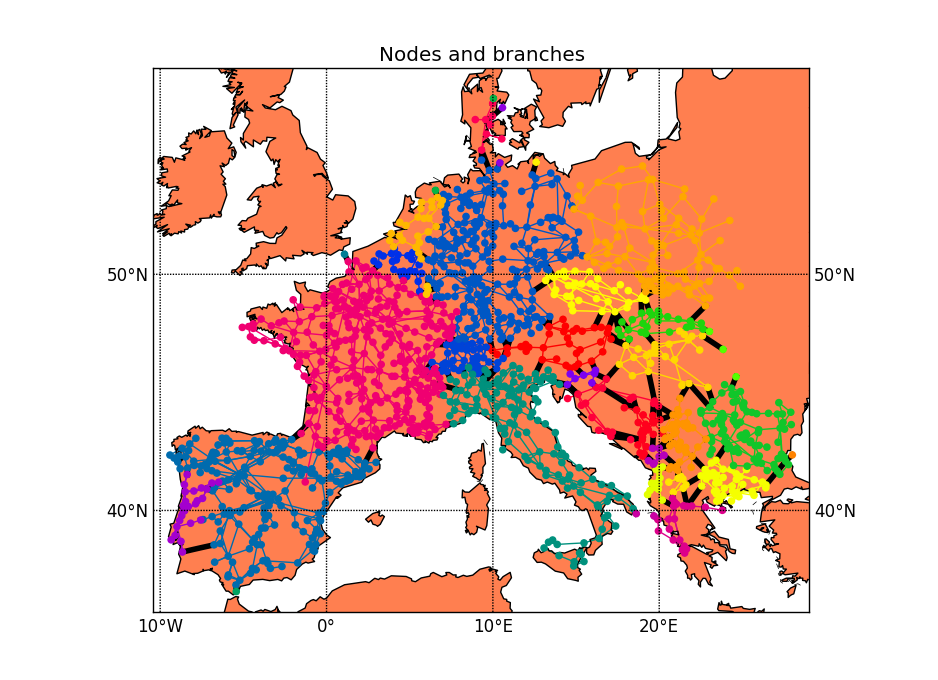
\includegraphics[scale=0.6]{example_2w_map_areas.png}
\caption{Power system included in analysis, coloured by area.}
\label{fig:example_map_areas}
\end{figure}

\begin{figure}
\centering
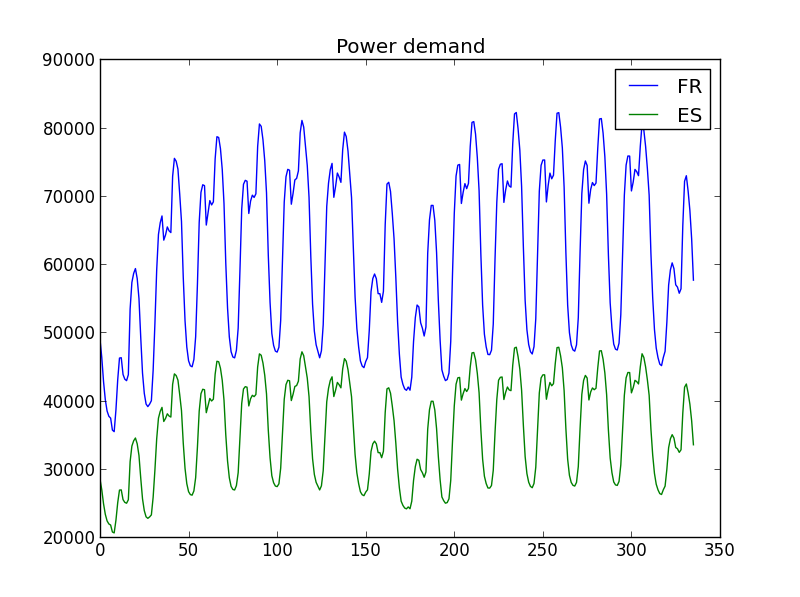
\includegraphics[scale=0.6]{example_2w_demand.png}
\caption{Power demand in France and Spain.}
\label{fig:example_demandl}
\end{figure}

\begin{figure}
\centering
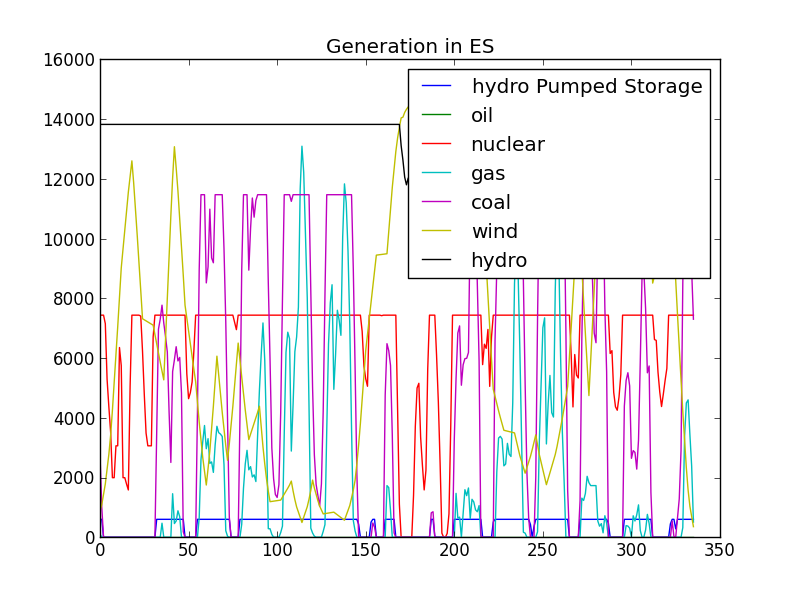
\includegraphics[scale=0.6]{example_2w_generationES.png}
\caption{Results: Power generation mix in Spain.}
\label{fig:example_generationES}
\end{figure}

\begin{figure}
\centering
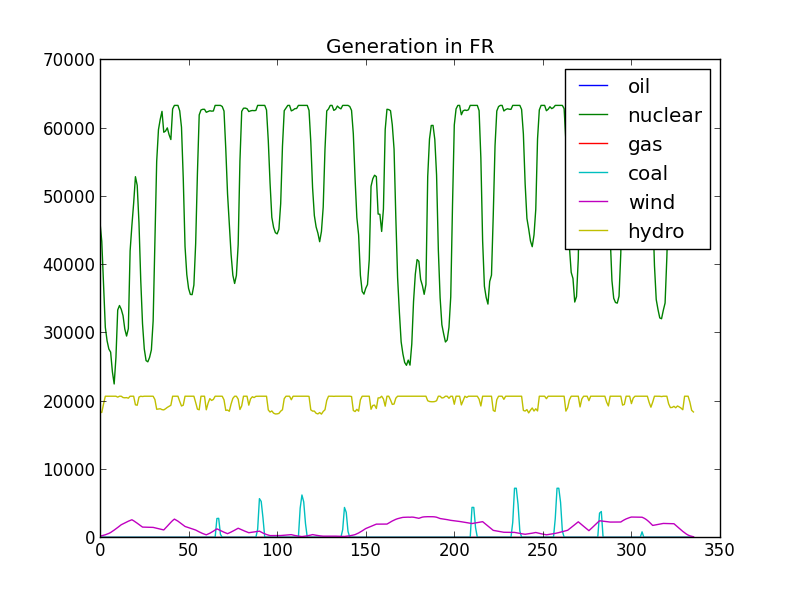
\includegraphics[scale=0.6]{example_2w_generationFR.png}
\caption{Results: Power generation mix in France.}
\label{fig:example_generationFR}
\end{figure}

\begin{figure}
\centering
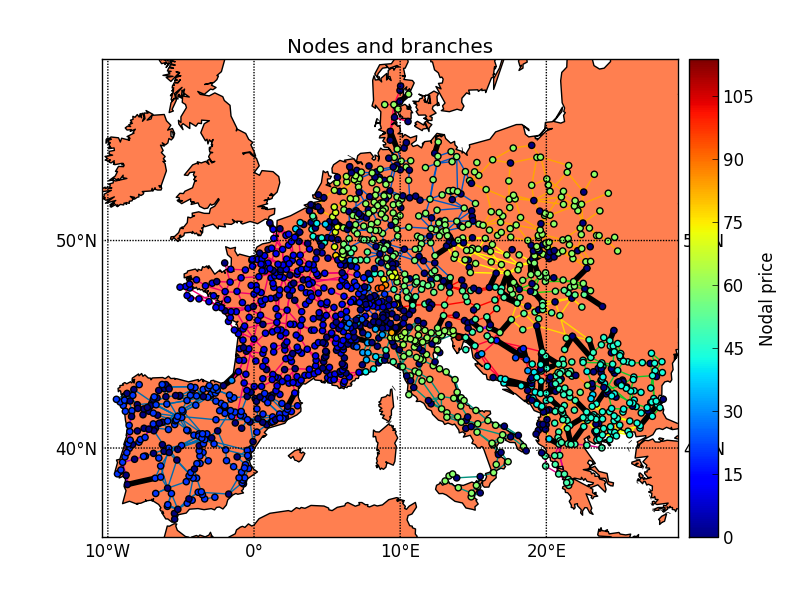
\includegraphics[scale=0.6]{example_2w_map_nodalprices.png}
\caption{Results: Average nodal prices. South-western Europe has lower prices due to relatively cheap nuclear power. }
\label{fig:example_map_prices}
\end{figure}



\newpage
\appendix

\section{Software design and implementation (TODO)}

\subsection{Class GridData}
nodes
branches
generators
consumers

\subsection{Class LpProblem}
This class contains the LP problem formulation using the PuLP interface. It contains the main loop that solves the problem for each time step and includes the dynamics that link the time steps.


\subsection{Class Results}
This class contains variables (arrays) with results for each time step, and methods to analyse and present the results.


\subsection{Implementation}
Python

Classes



\bibliographystyle{elsarticle-num}
%\bibliography{references}
%\bibliography{U:/prosjekt/500102_Elkraftsystemer/502000445_EU_EuroSunMed/Literature/bibliography_eurosunmed}
\bibliography{bibliography_eurosunmed}



\end{document}
